% =====================================================================
% Informe de avances - TP Senales (PSIB 16.63)
% Pre-procesamiento y extraccion de caracteristicas
%
% Compilar con pdflatex (o subir a Overleaf junto con la carpeta figuras/).
% Las figuras de figuras/ salen de resultados/figuras/ del repo.
% Donde dice [COMPLETAR] hay que actualizar con los registros elegidos.
% =====================================================================
\documentclass[11pt,a4paper]{article}

\usepackage[utf8]{inputenc}
\usepackage[T1]{fontenc}
\IfFileExists{lmodern.sty}{\usepackage{lmodern}}{}
\IfFileExists{spanish.ldf}
  {\usepackage[spanish,es-tabla,es-nodecimaldot]{babel}}
  {\renewcommand{\figurename}{Figura}\renewcommand{\tablename}{Tabla}
   \renewcommand{\refname}{Referencias}\renewcommand{\abstractname}{Resumen}}
\usepackage[margin=2.3cm]{geometry}
\usepackage{graphicx}
\usepackage{booktabs}
\usepackage{float}
\usepackage{caption}
\usepackage{amsmath}
\usepackage{xcolor}
\usepackage[colorlinks=true,linkcolor=blue!50!black,citecolor=blue!50!black,urlcolor=blue!60!black]{hyperref}

\graphicspath{{figuras/}}
\newcommand{\completar}[1]{\textcolor{red}{\textbf{[COMPLETAR: #1]}}}

\title{Detección de fibrilación auricular a partir de la serie RR\\[4pt]
\large Informe de avances: pre-procesamiento y extracción de características}
\author{\completar{integrantes} \\ Procesamiento de Señales e Imágenes Biomédicas (16.63) -- ITBA}
\date{Octubre de 2026}

\begin{document}
\maketitle

\begin{abstract}
Se presenta el avance del pipeline para detectar fibrilación auricular (FA) en registros Holter de 24~h de la base SHDB-AF sin usar aprendizaje automático. Se describen la selección de registros, la inspección espectral, el filtrado, la detección de segmentos ruidosos, la detección de QRS con Pan-Tompkins, la construcción y corrección de la serie RR, la segmentación en ventanas y la extracción de características temporales, de irregularidad y espectrales. Los resultados preliminares corresponden al registro 001 \completar{y a los registros elegidos}.
\end{abstract}

% ---------------------------------------------------------------------
\section{Introducción}
La FA es una taquiarritmia supraventricular con activación auricular descoordinada. En el ECG se caracteriza por intervalos R-R irregulares, ausencia de ondas P repetitivas y actividad auricular irregular~\cite{january2014}. El primer rasgo permite detectar FA solo a partir de la serie RR, lo que justifica el enfoque de este trabajo. La guía de 2014 fue actualizada por la de 2023~\cite{joglar2023}.

El objetivo es construir un detector sin aprendizaje automático: características calculadas por ventana y umbrales elegidos sobre un grupo de sujetos y evaluados sobre otro.

% ---------------------------------------------------------------------
\section{Base de datos}
Se usa SHDB-AF~\cite{tsutsui2025,shdbreadme}: 128 registros Holter de 24~h de 127 pacientes japoneses con FA paroxística. Cada registro tiene dos derivaciones (CC5 y NASA), grabadas a 125~Hz con un Holter Fukuda y remuestreadas a 200~Hz. Los encabezados de los archivos confirman $f_s = 200$~Hz y 2 canales (por ejemplo, el registro 001 tiene 17\,220\,000 muestras, 23,9~h).

Por registro hay cuatro archivos: \texttt{.hea} (encabezado), \texttt{.dat} (señal), \texttt{.qrs} (picos R detectados automáticamente con \textit{epltd}, una implementación de Pan-Tompkins) y \texttt{.atr} (anotaciones de ritmo latido a latido hechas a mano por un cardiólogo). El \texttt{.dat} es la entrada del pipeline; el \texttt{.qrs} se usa solo para validar la detección de QRS y el \texttt{.atr} solo como etiqueta, nunca como entrada del detector.

% ---------------------------------------------------------------------
\section{Metodología}
El código está en el repositorio del grupo (carpeta \texttt{codigo/}); todos los parámetros están centralizados en \texttt{config.py}.

\subsection{Etapa 0: selección de registros}
De los 128 registros, 98 tienen anotaciones de ritmo (\texttt{seleccion.py}). Se guarda el \texttt{Subject\_ID} de cada uno para que la partición train/test se haga por sujeto~\cite{dechazal2004}. Ninguno de los 98 tiene marcapasos durante el Holter. El pipeline se aplica a los 98 registros, de a 4 en paralelo (\texttt{correr\_todo.py}). \completar{registros que fallaron, si hubo}

\subsection{Etapa 1: carga por tramos}
Cada registro ocupa $\sim$69~MB y $17{,}2\times10^6$ muestras por canal. Se lee de a tramos de 30~min con 5~s de solape (para no perder latidos en los bordes) y se procesa el canal ECG1. La señal procesada no se guarda: solo los resultados (posiciones de R, serie RR, características).

\subsection{Etapa 2: inspección espectral}
Se estima la densidad espectral de potencia con el método de Welch~\cite{welch1967} (ventana de Hann de 10~s, 50\,\% de solape, resolución 0,1~Hz) en 6 tramos de 5~min repartidos en las 24~h.

\subsection{Etapa 3: filtrado y detección de ruido}
Se aplica un pasa-banda Butterworth de 0,5 a 40~Hz con \textit{filtfilt} (fase cero). El corte inferior elimina la deriva de línea de base; con filtrado de fase cero un corte de hasta 0,67~Hz no distorsiona el ECG~\cite{kligfield2007}. El corte superior atenúa el ruido muscular y el contenido por encima de 62,5~Hz. No se agrega notch (ver Sección~\ref{sec:res-espectro}).

Para detectar ruido se divide el registro en ventanas de 10~s y se calculan dos índices de calidad~\cite{li2008,clifford2012}:
\begin{itemize}
  \item \textbf{bSQI}: acuerdo entre dos detectores de QRS distintos (Pan-Tompkins y \texttt{xqrs} de la librería wfdb), $\text{bSQI} = \frac{VP}{VP+FN+FP}$ con tolerancia de 150~ms. Si el ECG está limpio, ambos detectores coinciden.
  \item \textbf{kSQI}: curtosis del ECG filtrado. Un ECG limpio es impulsivo (curtosis $>5$); el ruido tiende a una distribución gaussiana (curtosis $\approx 3$).
\end{itemize}
Una ventana se marca como ruidosa si $\text{bSQI} < 0{,}8$ o $\text{kSQI} < 5$. El umbral de bSQI es el que usan Chocron et al.~\cite{chocron2020} para excluir ventanas de 60 latidos en la detección de FA, tomado de Behar et al.~\cite{behar2013}; el de kSQI corresponde al valor por encima del cual un ECG sinusal se considera limpio~\cite{zhao2018}. \completar{ajuste de umbrales si se hizo}

\subsection{Etapa 4: limpieza con filtrado adaptativo (plan, sin implementar)}
Por ahora las ventanas ruidosas (etapa 3) se excluyen, que es lo que hacen trabajos de detección de FA a partir de la serie RR~\cite{chocron2020}. Como alternativa se plantea un mejorador adaptativo de línea (ALE)~\cite{widrow1975,thakor1991} aplicado solo a esas ventanas, para recuperar las que se puedan.

\textbf{Estructura.} El ALE es un cancelador de una sola entrada: la referencia es la propia señal retrasada $\Delta$ muestras, y un filtro FIR adaptativo de $L$ coeficientes predice la componente de la señal que sigue correlacionada después de $\Delta$; el ruido que se decorrelaciona en ese retardo queda en el error~\cite{widrow1975}. Thakor y Zhu~\cite{thakor1991} aplicaron estructuras adaptativas al ECG para cancelar ruido muscular y artefactos de movimiento, y una variante con referencia sincronizada con los QRS a la detección de FA.

\textbf{Limitación para FA.} El QRS tiene una duración del mismo orden que la correlación del ruido muscular, y en FA el RR es irregular, por lo que no puede usarse un retardo de un latido. La alternativa con referencia sincronizada a las R~\cite{thakor1991,fotiadou2018} depende de detectar bien las R, que es justamente lo que falla en las ventanas ruidosas. Esta limitación se evaluará antes de adoptar el ALE.

\textbf{Parámetros.} No hay en la literatura valores fijos de $\Delta$, $L$ y $\mu$ para este problema; en filtrado adaptativo de ECG se eligen por búsqueda sobre datos de prueba~\cite{fotiadou2018}. El plan es:

\begin{table}[H]
  \centering
  \small
  \caption{Diseño propuesto del ALE y fuente de cada parámetro.}
  \label{tab:ale}
  \begin{tabular}{p{2.6cm}p{6.6cm}p{3.6cm}}
    \toprule
    Parámetro & Valor o criterio & Fuente \\
    \midrule
    Estructura & ALE de una entrada, referencia = señal retrasada $\Delta$ & \cite{widrow1975} \\
    Algoritmo & LMS normalizado (NLMS), pesos iniciales en cero & \cite{fotiadou2018} \\
    Paso $\mu$ & Estabilidad: $0 < \mu < 2$ (NLMS); constante de tiempo $\tau \approx 1/(2\mu\lambda)$. Búsqueda en 8 valores logarítmicos entre 0,0005 y 0,1 & \cite{haykin2002,nosc1977,fotiadou2018} \\
    Coeficientes $L$ & Búsqueda en grilla (Fotiadou: 50 a 800 a 500~Hz; escalado a 200~Hz: 20 a 320) & \cite{fotiadou2018} \\
    Retardo $\Delta$ & Mayor que el ancho de la autocorrelación del ruido, medido en los registros \texttt{ma} y \texttt{em} de la NSTDB; menor que el de la autocorrelación del QRS & \cite{widrow1975,moody1984} \\
    Dónde se aplica & Solo en ventanas con bSQI $< 0{,}8$ o kSQI $< 5$ & \cite{chocron2020,zhao2018} \\
    Datos de prueba & ECG limpio + ruido \texttt{ma} y \texttt{em} de la MIT-BIH NSTDB a 24, 18, 12, 6, 0 y $-6$~dB & \cite{moody1984} \\
    Criterio de éxito & Mejora de $Se$ y $VPP$ de la detección de QRS (EC57) y recuperación de bSQI $\geq 0{,}8$; si no mejora, la ventana se excluye & \cite{ec57,chocron2020} \\
    \bottomrule
  \end{tabular}
\end{table}

Para controlar el sesgo, se reportará qué proporción de ventanas de FA y de no-FA queda excluida o recuperada.

\subsection{Etapa 5: detección de QRS}
Se usa el preprocesado de Pan y Tompkins~\cite{pantompkins1985}, diseñado para 200~Hz: pasa-banda de 5--15~Hz, derivada de 5 puntos, cuadrado e integración en ventana de 150~ms. Los filtros originales de coeficientes enteros se eligieron para operar en tiempo real en un microprocesador~\cite{pantompkins1985,hamilton1986}; como el procesamiento es \textit{offline}, se reemplazan por filtros Butterworth de orden 2 aplicados con \textit{filtfilt} (fase cero), como en Elgendi et al.~\cite{elgendi2010}, que usaron un Butterworth de segundo orden para comparar bandas de paso en la detección de QRS sobre MIT/BIH, y en línea con implementaciones de referencia que usan Butterworth de orden 1--2 para esta etapa~\cite{makowski2021}. Con fase cero no hay retardos que compensar.

Las reglas de decisión siguen la versión optimizada de Hamilton y Tompkins~\cite{hamilton1986}, que compararon cuantitativamente distintas reglas sobre la base MIT/BIH: niveles de QRS y de ruido estimados con la mediana de los últimos 8 picos (el mejor de los estimadores evaluados), umbral $DT = NPL + 0{,}1825\,(QRSPL - NPL)$, período refractario de 200~ms, búsqueda hacia atrás con la mitad del umbral si no hubo QRS en 1,5 veces la mediana de los últimos 8 RR, y descarte de ondas T entre 200 y 360~ms si la derivada máxima es menor a la mitad de la del QRS previo. Cada R se ubica en el máximo de $|\text{ECG}|$ en $\pm$100~ms alrededor de la detección.

La detección se valida contra el \texttt{.qrs} con la norma ANSI/AAMI EC57~\cite{ec57}: tolerancia de 150~ms, sensibilidad $Se = \frac{VP}{VP+FN}$ y valor predictivo positivo $VPP = \frac{VP}{VP+FP}$, solo dentro del tramo que cubre la referencia. Como el \texttt{.qrs} fue generado por \textit{epltd}, que implementa el mismo algoritmo de Hamilton y Tompkins, la referencia no es independiente: un acuerdo alto valida la implementación, no la detección en sí. Como referencia, Hamilton y Tompkins reportan $Se = 99{,}69\,\%$ y $VPP = 99{,}77\,\%$ en MIT/BIH~\cite{hamilton1986}.

\subsection{Etapa 6: serie RR y corrección}
Se calcula $RR_k = t_{k+1} - t_k$ y cada intervalo se marca como válido o inválido, sin borrarlo (para conservar la base temporal):
\begin{itemize}
  \item \textbf{fuera de rango}: $RR < 0{,}25$~s (falso QRS) o $RR > 2{,}5$~s (QRS perdido);
  \item \textbf{ruido}: el intervalo cae en una ventana ruidosa (etapa 3);
  \item \textbf{ectópico}: latido ectópico aislado y su pausa compensatoria, con el criterio de Dash et al.~\cite{dash2009}: $RR_i/RR_{i-1}$ en el percentil 1, $RR_{i+1}/RR_i$ en el percentil 99 y $RR_{i+1}/RR_{i+2}$ por encima del percentil 25. Dash et al. reportan que remover ectópicos aislados sube la especificidad de 69,4\,\% a 91,2\,\%;
  \item \textbf{transición}: el intervalo cruza un cambio de ritmo.
\end{itemize}
No se descartan intervalos por ser irregulares, ya que la irregularidad es justamente lo que caracteriza a la FA. Las ideas de prefiltrado de la serie RR siguen a PhysioZoo~\cite{behar2018}, la herramienta usada para anotar SHDB-AF.

\subsection{Etapa 7: ventanas}
La serie RR se divide en ventanas de 60 intervalos consecutivos sin solape, el largo usado en el benchmark de SHDB-AF~\cite{tsutsui2025}. En la literatura se usan desde 8~\cite{petrenas2015} y 12~\cite{lake2011} hasta 128 latidos~\cite{dash2009}. Se conservan solo las ventanas con una única etiqueta (FA o no-FA) y al menos 90\,\% de intervalos válidos. Flúter y otras taquicardias auriculares se excluyen. \completar{comparación 60 vs 128 latidos}

\subsection{Etapa 8: características por ventana}
Sobre los intervalos válidos de cada ventana se calculan:
\begin{itemize}
  \item \textbf{Temporales}~\cite{taskforce1996}: media RR, SDNN y RMSSD.
  \item \textbf{Irregularidad}~\cite{dash2009,lake2011}: RMSSD normalizado por la media (nRMSSD), \textit{turning point ratio} (TPR, fracción de máximos y mínimos locales; vale $\approx 2/3$ en una serie aleatoria), entropía de Shannon del histograma de RR (16 bins, sin los 8 RR más largos ni los 8 más cortos, normalizada a $[0,1]$) y entropía muestral ($m=2$, $r = 0{,}2\,\sigma$).
  \item \textbf{Espectrales}: potencia relativa en LF (0,04--0,15~Hz) y HF (0,15--0,4~Hz) y cociente LF/HF con el periodograma de Lomb~\cite{laguna1998}, que no requiere muestras equiespaciadas. El Task Force recomienda registros de 5~min para el análisis espectral de corto plazo y al menos $\sim$2~min para LF~\cite{taskforce1996,shaffer2017}; con ventanas de $\sim$1~min, LF no es confiable y en FA estas bandas no reflejan modulación autonómica. Se reportan como medidas de irregularidad. Como comparación se plantea una PSD paramétrica AR (Yule-Walker, orden por AIC/BIC~\cite{boardman2002}). \completar{AR si se implementa}
\end{itemize}

% ---------------------------------------------------------------------
\section{Resultados preliminares}
Los resultados corresponden al registro 001: 809~min de FA seguidos de 626~min de ritmo no-FA, sin marcapasos. \completar{agregar los demás registros}

\subsection{Espectro}\label{sec:res-espectro}
La Figura~\ref{fig:espectro} muestra la PSD. El 99,8\,\% de la potencia cae entre 0,5 y 40~Hz. Se observan dos pozos: en 50~Hz, que indica que el Holter ya aplica un notch de red, y en 75~Hz, que es el reflejo de ese notch por el remuestreo de 125 a 200~Hz ($125 - 50 = 75$~Hz). Por el mismo motivo, el contenido por encima de 62,5~Hz es un artefacto del remuestreo (0,08\,\% de la potencia), que el pasa-bajos de 40~Hz elimina. No hace falta agregar un notch.

\begin{figure}[H]
  \centering
  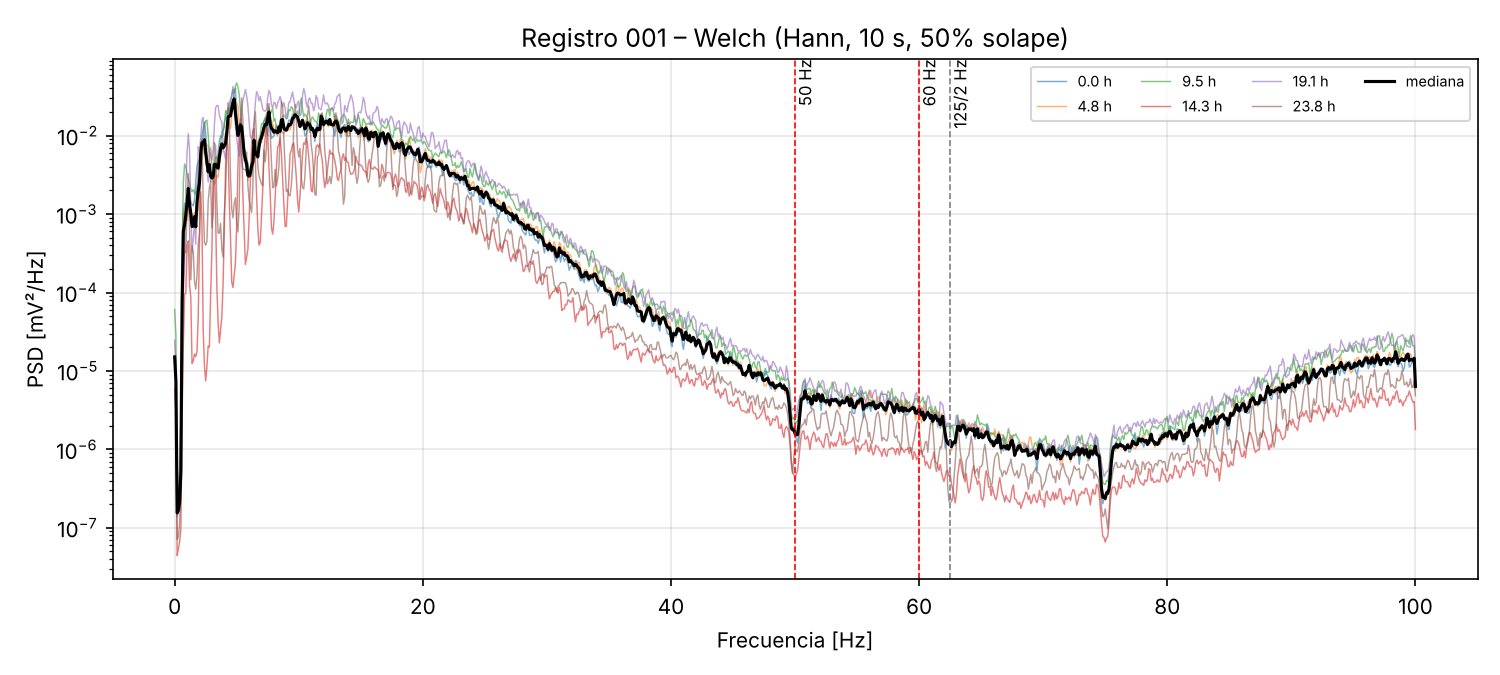
\includegraphics[width=0.9\linewidth]{espectro_001.png}
  \caption{PSD de Welch del registro 001 en 6 tramos de 5~min y su mediana. Líneas: 50, 60 y 62,5~Hz.}
  \label{fig:espectro}
\end{figure}

\subsection{Filtrado y ruido}
La Figura~\ref{fig:filtrado} muestra el efecto del pasa-banda. En el registro 001 ninguna de las 8610 ventanas de 10~s se marcó como ruidosa: el bSQI mínimo fue 0,90 y el kSQI mínimo 6,05 (Figura~\ref{fig:ruido}). Los umbrales todavía deben ponerse a prueba en registros con ruido. \completar{resultados en otros registros}

\begin{figure}[H]
  \centering
  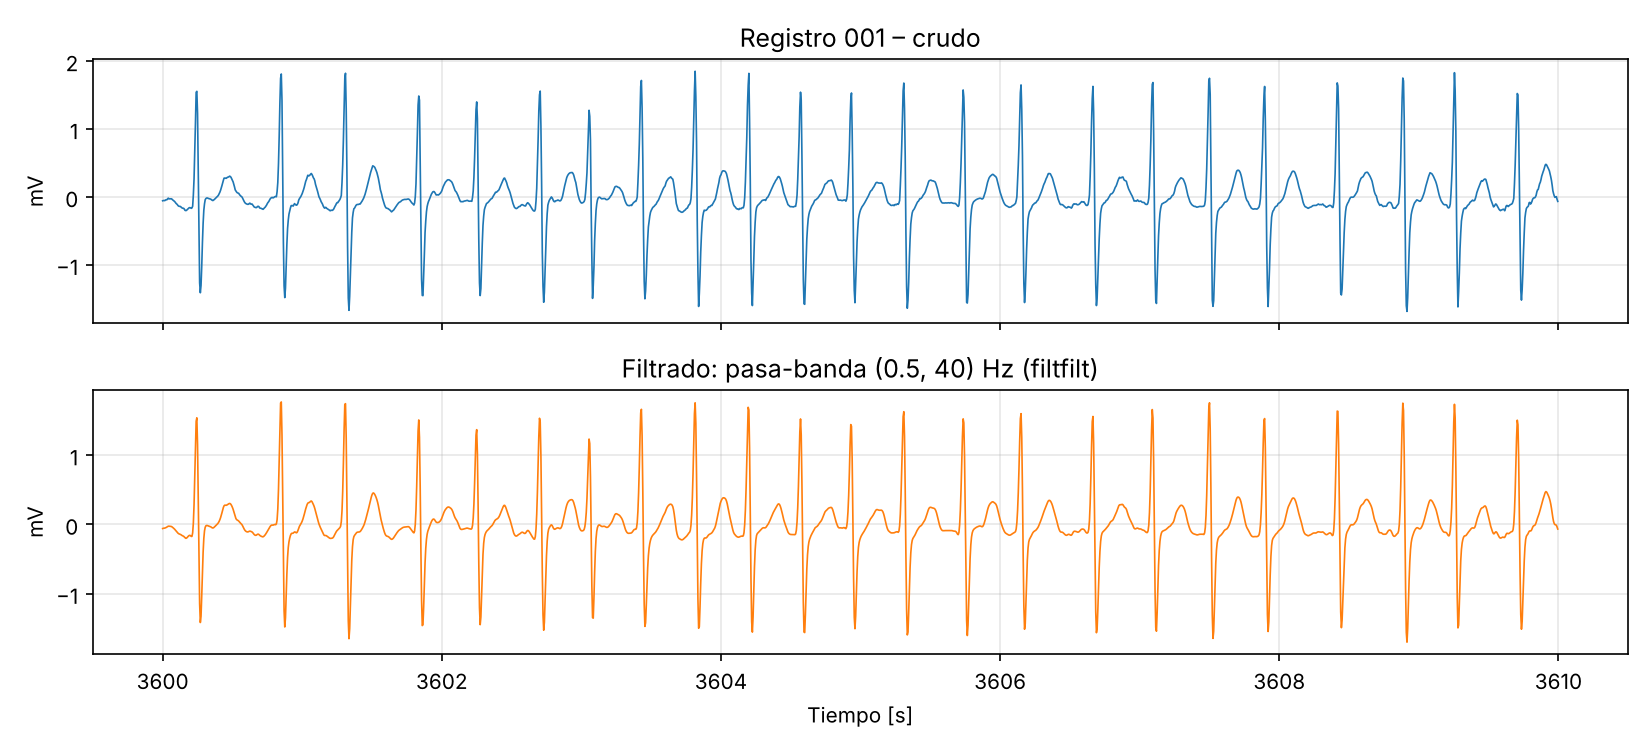
\includegraphics[width=0.9\linewidth]{filtrado_001.png}
  \caption{ECG crudo (arriba) y filtrado con pasa-banda de 0,5--40~Hz (abajo).}
  \label{fig:filtrado}
\end{figure}

\begin{figure}[H]
  \centering
  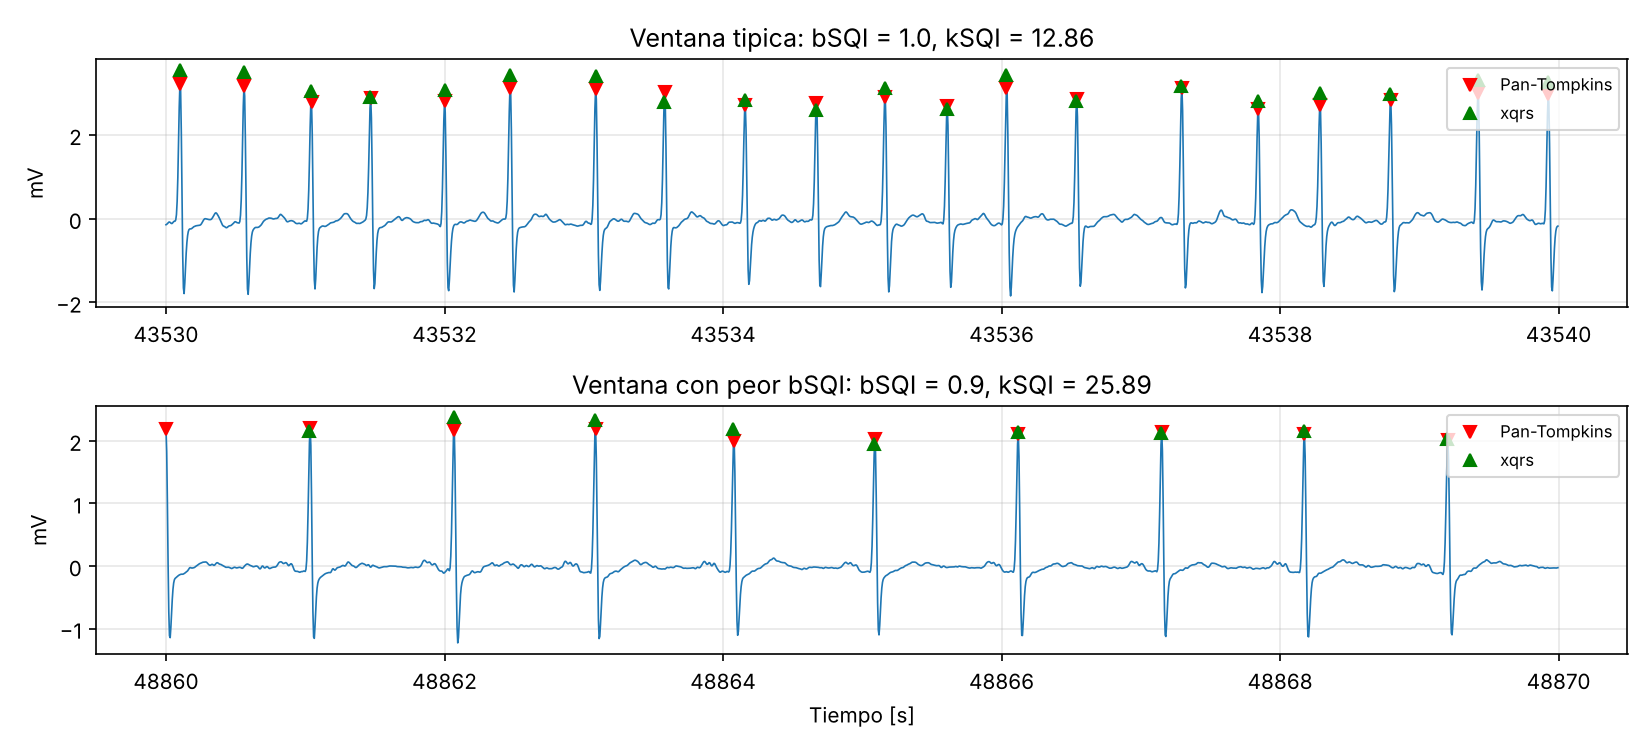
\includegraphics[width=0.9\linewidth]{ruido_001.png}
  \caption{Ventana típica y ventana de peor bSQI, con las detecciones de Pan-Tompkins y \texttt{xqrs}. El bSQI de 0,9 se debe a un latido en el borde de la ventana, no a ruido.}
  \label{fig:ruido}
\end{figure}

\subsection{Detección de QRS}
\begin{table}[H]
  \centering
  \caption{Validación de Pan-Tompkins contra el \texttt{.qrs} (tolerancia 150~ms).}
  \label{tab:qrs}
  \begin{tabular}{lrrrrr}
    \toprule
    Registro & VP & FN & FP & $Se$ (\%) & $VPP$ (\%) \\
    \midrule
    001 & 143\,768 & 0 & 0 & 100,00 & 100,00 \\
    \completar{} & & & & & \\
    \bottomrule
  \end{tabular}
\end{table}

\begin{figure}[H]
  \centering
  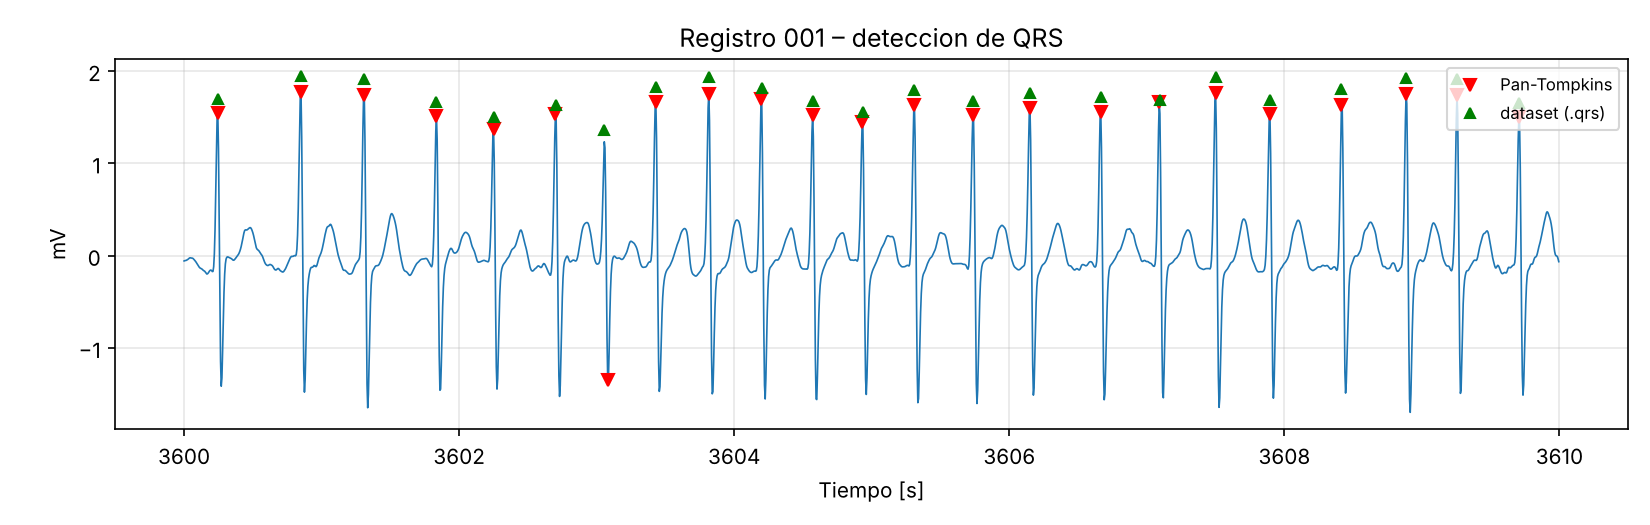
\includegraphics[width=0.9\linewidth]{qrs_001.png}
  \caption{Detecciones propias y del dataset sobre 10~s del registro 001.}
  \label{fig:qrs}
\end{figure}

\subsection{Serie RR}
El registro 001 tiene 143\,786 intervalos, de los cuales el 99,6\,\% son válidos: 1 fuera de rango, 516 marcados como ectópicos y 1 en la transición de ritmo. En la Figura~\ref{fig:tacograma} se ve el cambio de FA (RR cortos, $\approx$0,45~s, y muy dispersos) a no-FA (RR $\approx$0,9~s y ordenados). Parte de los intervalos marcados como ectópicos cae dentro de la FA. \completar{comparación con y sin remoción de ectópicos}

\begin{figure}[H]
  \centering
  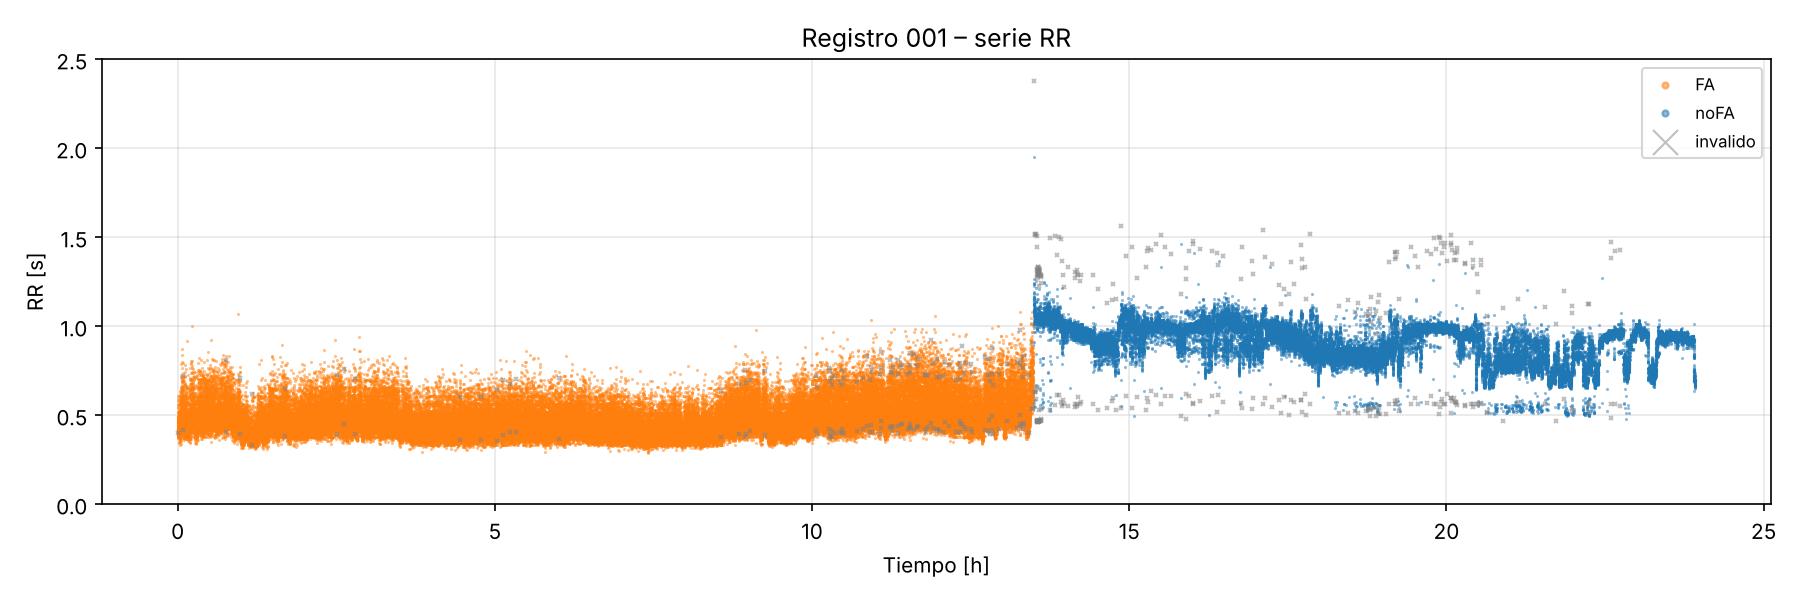
\includegraphics[width=\linewidth]{tacograma_001.png}
  \caption{Serie RR de las 24~h del registro 001. Naranja: FA; azul: no-FA; gris: intervalos inválidos.}
  \label{fig:tacograma}
\end{figure}

\subsection{Características}
Se obtuvieron 2389 ventanas de 60 latidos (1702 de FA y 687 de no-FA). La Tabla~\ref{tab:caract} y la Figura~\ref{fig:boxplots} muestran que las medidas de irregularidad separan bien ambas clases: la mediana de nRMSSD es 0,20 en FA y 0,04 en no-FA, y la de TPR 0,58 y 0,42, consistentes con los umbrales de Dash et al. (nRMSSD $> 0{,}1$; TPR entre 0,54 y 0,77)~\cite{dash2009}. LF/HF casi no separa, como se esperaba con ventanas cortas.

\begin{table}[H]
  \centering
  \caption{Mediana de cada característica por clase (registro 001).}
  \label{tab:caract}
  \begin{tabular}{lrr}
    \toprule
    Característica & no-FA & FA \\
    \midrule
    Media RR (s)   & 0,925 & 0,466 \\
    SDNN (s)       & 0,043 & 0,072 \\
    RMSSD (s)      & 0,033 & 0,094 \\
    nRMSSD         & 0,037 & 0,202 \\
    TPR            & 0,417 & 0,583 \\
    Shannon        & 0,836 & 0,901 \\
    SampEn         & 1,19  & 1,95  \\
    LF (relativa)  & 0,172 & 0,222 \\
    HF (relativa)  & 0,349 & 0,503 \\
    LF/HF          & 0,543 & 0,449 \\
    \bottomrule
  \end{tabular}
\end{table}

\begin{figure}[H]
  \centering
  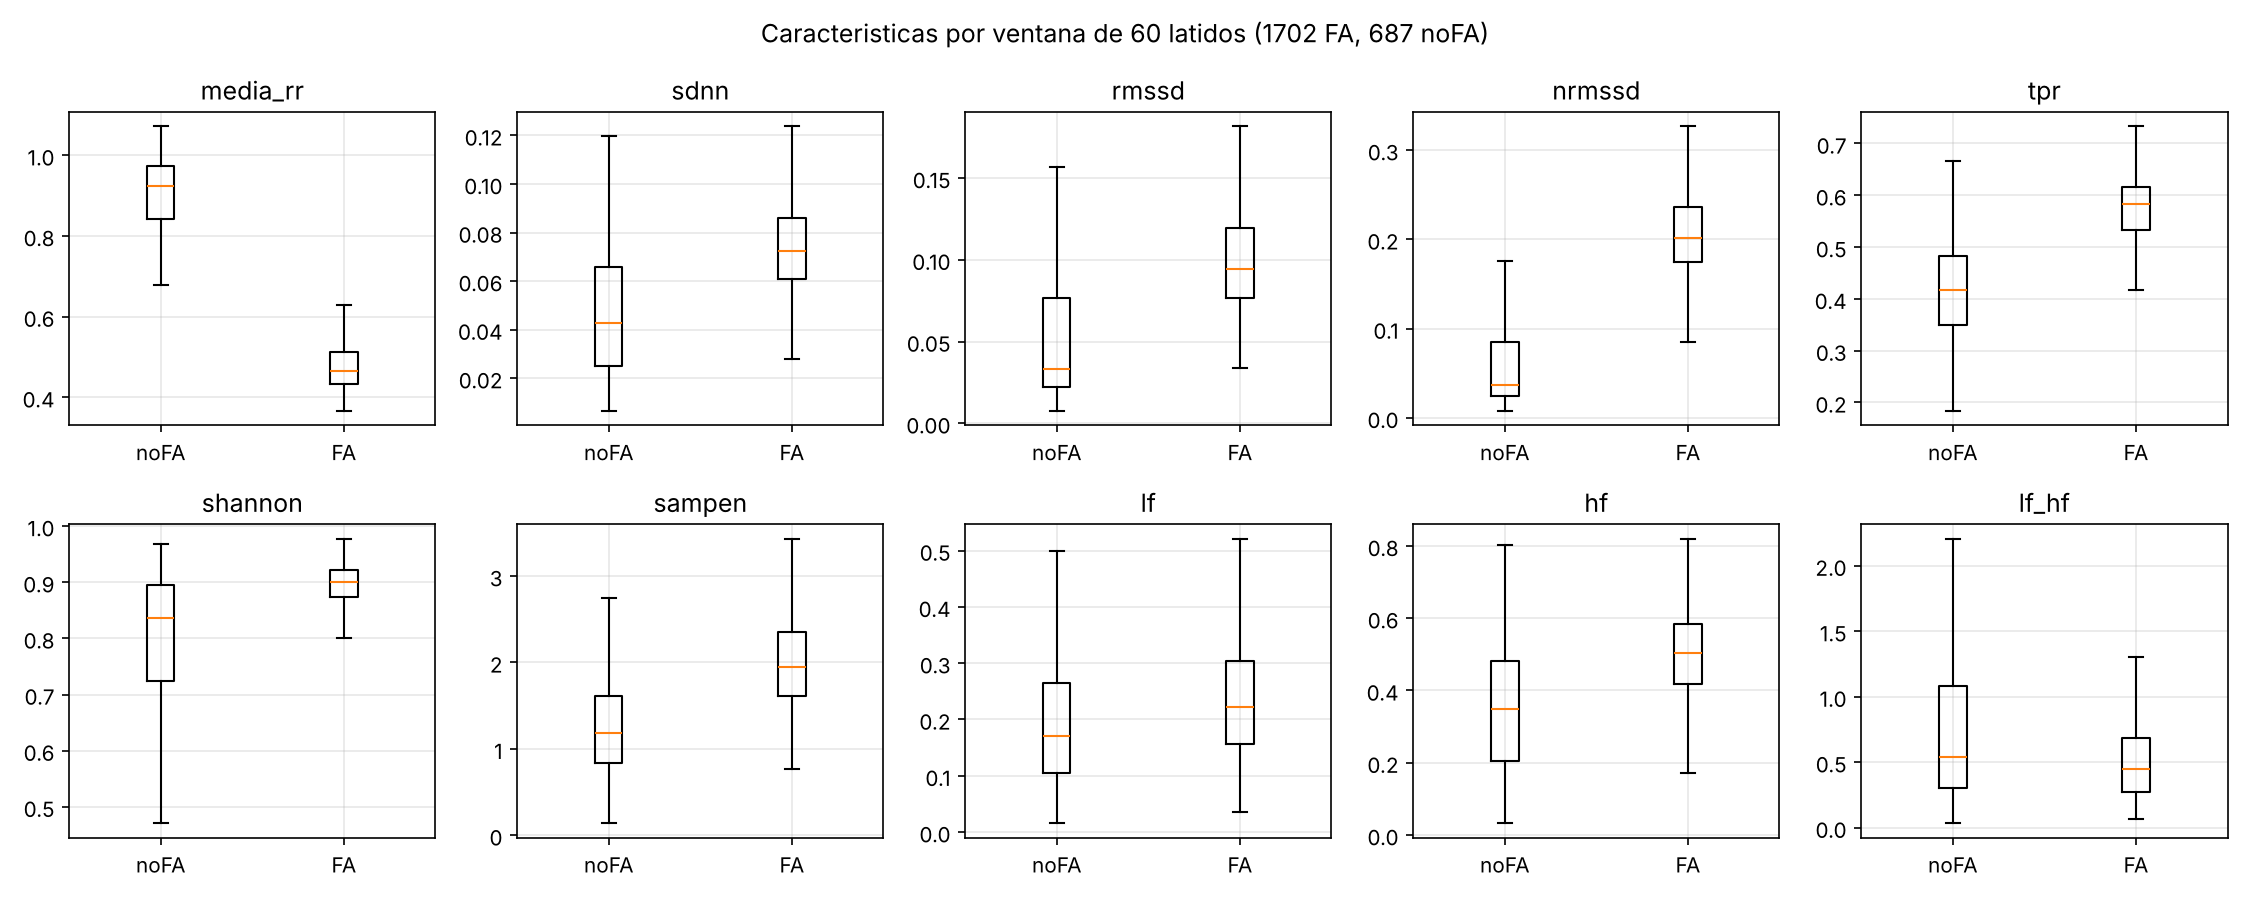
\includegraphics[width=\linewidth]{boxplots_caracteristicas.png}
  \caption{Distribución de cada característica por clase (sin valores atípicos).}
  \label{fig:boxplots}
\end{figure}

% ---------------------------------------------------------------------
\section{Limitaciones y próximos pasos}
\begin{itemize}
  \item Los resultados son de un solo registro: falta procesar los 98 registros anotados.
  \item Los umbrales de ruido no se probaron en registros ruidosos, y el ALE (etapa 4) está pendiente.
  \item La regla de ectópicos marca algunos intervalos dentro de la FA; hay que evaluar su efecto.
  \item Las ventanas de un mismo sujeto no son independientes: la estadística (etapa 9) se hará con valores agregados por sujeto y con corrección por comparaciones múltiples.
  \item Etapa 9: curva ROC y AUC por característica, umbral elegido en un grupo de sujetos (train) y evaluado en otro (test), con sensibilidad y especificidad.
\end{itemize}

% ---------------------------------------------------------------------
\begin{thebibliography}{99}

\bibitem{tsutsui2025} K.~Tsutsui, S.~Biton Brimer, N.~Ben-Moshe, et al., ``SHDB-AF: a Japanese Holter ECG database of atrial fibrillation,'' \textit{Scientific Data}, vol.~12, 2025. \url{https://doi.org/10.1038/s41597-025-04777-4}

\bibitem{shdbreadme} SHDB-AF v1.0.1, PhysioNet. \url{https://physionet.org/content/shdb-af/1.0.1/}

\bibitem{january2014} C.~T.~January, L.~S.~Wann, J.~S.~Alpert, et al., ``2014 AHA/ACC/HRS guideline for the management of patients with atrial fibrillation,'' \textit{J. Am. Coll. Cardiol.}, vol.~64, no.~21, pp.~e1--e76, 2014. \url{https://doi.org/10.1016/j.jacc.2014.03.022}

\bibitem{joglar2023} J.~A.~Joglar, M.~K.~Chung, et al., ``2023 ACC/AHA/ACCP/HRS guideline for the diagnosis and management of atrial fibrillation,'' \textit{Circulation}, vol.~149, 2024. \completar{verificar cita}

\bibitem{dechazal2004} P.~de~Chazal, M.~O'Dwyer, R.~B.~Reilly, ``Automatic classification of heartbeats using ECG morphology and heartbeat interval features,'' \textit{IEEE Trans. Biomed. Eng.}, vol.~51, no.~7, pp.~1196--1206, 2004. \url{https://doi.org/10.1109/TBME.2004.827359}

\bibitem{welch1967} P.~D.~Welch, ``The use of fast Fourier transform for the estimation of power spectra,'' \textit{IEEE Trans. Audio Electroacoust.}, vol.~15, no.~2, pp.~70--73, 1967. \url{https://doi.org/10.1109/TAU.1967.1161901}

\bibitem{kligfield2007} P.~Kligfield, L.~S.~Gettes, J.~J.~Bailey, et al., ``Recommendations for the standardization and interpretation of the electrocardiogram: Part I,'' \textit{Circulation}, vol.~115, pp.~1306--1324, 2007. \url{https://doi.org/10.1161/CIRCULATIONAHA.106.180200}

\bibitem{li2008} Q.~Li, R.~G.~Mark, G.~D.~Clifford, ``Robust heart rate estimation from multiple asynchronous noisy sources using signal quality indices and a Kalman filter,'' \textit{Physiol. Meas.}, vol.~29, pp.~15--32, 2008. \url{https://doi.org/10.1088/0967-3334/29/1/002}

\bibitem{clifford2012} G.~D.~Clifford, J.~Behar, Q.~Li, I.~Rezek, ``Signal quality indices and data fusion for determining clinical acceptability of electrocardiograms,'' \textit{Physiol. Meas.}, vol.~33, pp.~1419--1433, 2012. \url{https://doi.org/10.1088/0967-3334/33/9/1419}

\bibitem{behar2013} J.~Behar, J.~Oster, Q.~Li, G.~D.~Clifford, ``ECG signal quality during arrhythmia and its application to false alarm reduction,'' \textit{IEEE Trans. Biomed. Eng.}, vol.~60, no.~6, pp.~1660--1666, 2013. \url{https://doi.org/10.1109/TBME.2013.2240452}

\bibitem{chocron2020} A.~Chocron, R.~Efraim, F.~Mandel, et al., J.~A.~Behar, ``Digital biomarkers and artificial intelligence for mass diagnosis of atrial fibrillation in a population sample at risk of sleep disordered breathing,'' arXiv:2007.14686, 2020. \url{https://arxiv.org/abs/2007.14686}

\bibitem{zhao2018} Z.~Zhao, Y.~Zhang, ``SQI quality evaluation mechanism of single-lead ECG signal based on simple heuristic fusion and fuzzy comprehensive evaluation,'' \textit{Front. Physiol.}, vol.~9, 727, 2018. \url{https://doi.org/10.3389/fphys.2018.00727}

\bibitem{widrow1975} B.~Widrow, J.~R.~Glover, J.~M.~McCool, et al., ``Adaptive noise cancelling: principles and applications,'' \textit{Proc. IEEE}, vol.~63, no.~12, pp.~1692--1716, 1975. \url{https://doi.org/10.1109/PROC.1975.10036}

\bibitem{nosc1977} Naval Ocean Systems Center, ``Adaptive noise cancelling and enhancement of a sinusoid in uncorrelated noise,'' Technical Report 184, 1977. \url{https://apps.dtic.mil/sti/pdfs/ADA050313.pdf}

\bibitem{haykin2002} S.~Haykin, \textit{Adaptive Filter Theory}, 4.ª ed. Upper Saddle River, NJ: Prentice Hall, 2002.

\bibitem{fotiadou2018} E.~Fotiadou, J.~O.~E.~H.~van~Laar, S.~G.~Oei, R.~Vullings, ``Enhancement of low-quality fetal electrocardiogram based on time-sequenced adaptive filtering,'' \textit{Med. Biol. Eng. Comput.}, vol.~56, 2018. \url{https://doi.org/10.1007/s11517-018-1862-8}

\bibitem{moody1984} G.~B.~Moody, W.~E.~Muldrow, R.~G.~Mark, ``A noise stress test for arrhythmia detectors,'' \textit{Computers in Cardiology}, vol.~11, pp.~381--384, 1984. Base: \url{https://physionet.org/content/nstdb/1.0.0/}

\bibitem{thakor1991} N.~V.~Thakor, Y.~S.~Zhu, ``Applications of adaptive filtering to ECG analysis: noise cancellation and arrhythmia detection,'' \textit{IEEE Trans. Biomed. Eng.}, vol.~38, no.~8, pp.~785--794, 1991.

\bibitem{pantompkins1985} J.~Pan, W.~J.~Tompkins, ``A real-time QRS detection algorithm,'' \textit{IEEE Trans. Biomed. Eng.}, vol.~32, no.~3, pp.~230--236, 1985. \url{https://doi.org/10.1109/TBME.1985.325532}

\bibitem{hamilton1986} P.~S.~Hamilton, W.~J.~Tompkins, ``Quantitative investigation of QRS detection rules using the MIT/BIH arrhythmia database,'' \textit{IEEE Trans. Biomed. Eng.}, vol.~BME-33, no.~12, pp.~1157--1165, 1986.

\bibitem{elgendi2010} M.~Elgendi, M.~Jonkman, F.~De~Boer, ``Frequency bands effects on QRS detection,'' en \textit{Proc. 3rd Int. Conf. Bio-inspired Systems and Signal Processing (BIOSIGNALS)}, pp.~428--431, 2010.

\bibitem{makowski2021} D.~Makowski, T.~Pham, Z.~J.~Lau, et al., ``NeuroKit2: A Python toolbox for neurophysiological signal processing,'' \textit{Behav. Res. Methods}, vol.~53, no.~4, pp.~1689--1696, 2021. \url{https://doi.org/10.3758/s13428-020-01516-y}

\bibitem{ec57} ANSI/AAMI EC57, \textit{Testing and reporting performance results of cardiac rhythm and ST segment measurement algorithms}. \url{https://webstore.ansi.org/standards/aami/ansiaamiisoec571998r2008}

\bibitem{dash2009} S.~Dash, K.~H.~Chon, S.~Lu, E.~A.~Raeder, ``Automatic real time detection of atrial fibrillation,'' \textit{Ann. Biomed. Eng.}, vol.~37, no.~9, pp.~1701--1709, 2009. \url{https://doi.org/10.1007/s10439-009-9740-z}

\bibitem{behar2018} J.~A.~Behar, A.~A.~Rosenberg, I.~Weiser-Bitoun, et al., ``PhysioZoo: a novel open access platform for heart rate variability analysis of mammalian electrocardiographic data,'' \textit{Front. Physiol.}, vol.~9, 2018. \url{https://doi.org/10.3389/fphys.2018.01390}

\bibitem{petrenas2015} A.~Petrėnas, V.~Marozas, L.~Sörnmo, ``Low-complexity detection of atrial fibrillation in continuous long-term monitoring,'' \textit{Comput. Biol. Med.}, vol.~65, pp.~184--191, 2015. \url{https://doi.org/10.1016/j.compbiomed.2015.01.019}

\bibitem{lake2011} D.~E.~Lake, J.~R.~Moorman, ``Accurate estimation of entropy in very short physiological time series: the problem of atrial fibrillation detection in implanted ventricular devices,'' \textit{Am. J. Physiol. Heart Circ. Physiol.}, vol.~300, pp.~H319--H325, 2011.

\bibitem{taskforce1996} Task Force of the ESC and NASPE, ``Heart rate variability: standards of measurement, physiological interpretation and clinical use,'' \textit{Circulation}, vol.~93, pp.~1043--1065, 1996. \url{https://doi.org/10.1161/01.CIR.93.5.1043}

\bibitem{shaffer2017} F.~Shaffer, J.~P.~Ginsberg, ``An overview of heart rate variability metrics and norms,'' \textit{Front. Public Health}, vol.~5, 258, 2017. \url{https://doi.org/10.3389/fpubh.2017.00258}

\bibitem{laguna1998} P.~Laguna, G.~B.~Moody, R.~G.~Mark, ``Power spectral density of unevenly sampled data by least-square analysis: performance and application to heart rate signals,'' \textit{IEEE Trans. Biomed. Eng.}, vol.~45, no.~6, pp.~698--715, 1998. \url{https://doi.org/10.1109/10.678605}

\bibitem{boardman2002} A.~Boardman, F.~S.~Schlindwein, A.~P.~Rocha, A.~Leite, ``A study on the optimum order of autoregressive models for heart rate variability,'' \textit{Physiol. Meas.}, vol.~23, pp.~325--336, 2002.

\end{thebibliography}

\end{document}
